\section{信息率失真函数}
\label{sec:rd-information-rd}

$R_{\mathrm{op}}(D)$的定义涉及所有块长、所有码本，无法直接计算。我们需要一个只看单个符号就能算的量，并且它要与码的描述能力挂钩。互信息正好起这个作用。

设$(n,M)$码的重构块为$\hat{X}^{n}=g_n(f_n(X^{n}))$。它由编号决定，至多取$M$个值，所以它能携带的关于$X^{n}$的信息有限：
\[
  I(X^{n};\hat{X}^{n})\leq H(\hat{X}^{n})\leq\log_2M=nR .
\]
第一个不等号来自
\[
  I(X^{n};\hat{X}^{n})=H(\hat{X}^{n})-H(\hat{X}^{n}\mid X^{n})
\]
与条件熵非负，第二个是取$M$个值的变量熵不超过$\log_2M$。所以码率至少要容纳重构与源之间的互信息。重构必须足够接近源，这又迫使互信息不能太小。下面在单个符号上精确地表述这种张力：失真不超过$D$时，互信息最少是多少。

这里沿用第~\ref{chap:information-measures}章的熵、条件熵与互信息，只把对数换成以$2$为底，数值都除以$\ln2$，单位从nat变成bit。有限字母表上，
\[
  I(X;\hat{X})=\sum_{x,\hat{x}}p(x,\hat{x})\log_2\frac{p(x,\hat{x})}{p(x)\,r(\hat{x})},
\]
其中$r$是$\hat{X}$的分布；它就是联合分布相对边缘乘积的KL散度，非负，且为零当且仅当$X$与$\hat{X}$独立。

\subsection{重构条件分布}
\label{sec:rd-test-channels}

单个符号上，一个“重构规律”就是给定源值$x$时，重构值怎样选择。允许这种选择带有随机性，用条件分布描述它。

设$\mathcal{X}$与$\hat{\mathcal{X}}$是有限集，$p(x)=P_X(\{x\})$。一个\term{测试信道}（test channel）是一族条件概率$q(\hat{x}\mid x)\geq0$，对每个$x$有$\sum_{\hat{x}}q(\hat{x}\mid x)=1$。它与源分布一起确定联合分布$p(x)q(\hat{x}\mid x)$，重构的边缘分布是
\begin{equation}
  r_q(\hat{x})=\sum_{x}p(x)\,q(\hat{x}\mid x).
  \label{eq:rd-output-marginal}
\end{equation}
把$q$看作一个随机的“重构器”：输入$x$，按$q(\cdot\mid x)$抽一个$\hat{x}$输出。它的平均失真与互信息分别是
\begin{equation}
  \mathbb{E}d(X,\hat{X})=\sum_{x,\hat{x}}p(x)\,q(\hat{x}\mid x)\,d(x,\hat{x}),
  \label{eq:rd-test-distortion}
\end{equation}
\begin{equation}
  I(P_X,q)=\sum_{x,\hat{x}}p(x)\,q(\hat{x}\mid x)\log_2\frac{q(\hat{x}\mid x)}{r_q(\hat{x})}.
  \label{eq:rd-test-information}
\end{equation}
式~\eqref{eq:rd-test-information}中约定$0\log_20=0$；若$p(x)q(\hat{x}\mid x)>0$，则$r_q(\hat{x})>0$，分母不会为零。

\begin{definition}[信息率失真函数]
\label{def:rd-information-rd}
给定源分布$P_X$与失真函数$d$，对$D\geq0$令
\begin{equation}
  R(D)=\inf\Bigl\{I(P_X,q):\ q\text{为测试信道},\ \mathbb{E}d(X,\hat{X})\leq D\Bigr\},
  \label{eq:rd-information-rd}
\end{equation}
约定空集的下确界为$+\infty$。$R(D)$称为\term{信息率失真函数}（information rate-distortion function），单位是bit每源符号。
\end{definition}

式~\eqref{eq:rd-information-rd}的优化变量只有测试信道$q$。源分布$P_X$是给定的，不参与优化；改变的只是“看到$x$以后怎样重构”。下一部分研究信道时问题方向相反：信道的条件分布固定，改变的是输入分布。两个问题都优化互信息，但一个求最小、一个求最大，变量也不同。

测试信道是一个理论对象，不是编码器。真正的编码器看到整块源符号，确定地输出一个编号；测试信道只作用在单个符号上，并且允许抛硬币。它在本章有两个用处：在第~\ref{sec:rd-coding-theorem}节的下界证明中，任意块编码都会诱导出一个测试信道；在可达性证明中，最优测试信道指导怎样随机生成码本。$R(D)$与$R_{\mathrm{op}}(D)$相等是需要证明的定理，现在只把$R(D)$当作一个优化问题来研究。

一般的取值空间中，测试信道是从$\mathcal{X}$到$\hat{\mathcal{X}}$的Markov核（第~\ref{chap:conditional-distributions}章），互信息用联合分布相对边缘乘积的KL散度定义，允许取$+\infty$，式~\eqref{eq:rd-information-rd}的写法不变。本节余下部分先在有限字母表上讨论，一般情形放在第~\ref{sec:rd-feasible-range}节末尾。

\paragraph{三个测试信道}
仍取$X\sim\operatorname{Bern}(0.3)$与Hamming失真。第一个测试信道不看输入，一律输出$0$。这时$\hat{X}$是常数，与$X$独立，
\[
  I=0,\qquad \mathbb{E}d=\mathbb{P}(X=1)=0.3 .
\]

第二个测试信道以概率$0.1$把输入翻转：$q(1\mid0)=q(0\mid1)=0.1$。平均失真正好是翻转概率$0.1$。由式~\eqref{eq:rd-output-marginal}，
\[
  r_q(1)=0.7\times0.1+0.3\times0.9=0.34 .
\]
给定$X$时$\hat{X}$的熵是$h_2(0.1)$，于是
\[
  I=H(\hat{X})-H(\hat{X}\mid X)=h_2(0.34)-h_2(0.1)\approx0.9248-0.4690=0.4558 .
\]

第三个测试信道取$q(1\mid0)=\tfrac1{28}$，$q(0\mid1)=\tfrac14$：常见的$0$几乎不动，罕见的$1$有四分之一被改成$0$。平均失真仍然是
\[
  \mathbb{E}d=0.7\times\frac{1}{28}+0.3\times\frac14=0.025+0.075=0.1 .
\]
重构边缘为
\[
  r_q(1)=0.7\times\frac1{28}+0.3\times\frac34=0.25 .
\]

给定$X=0$与$X=1$时$\hat{X}$的熵分别是$h_2(\tfrac1{28})$与$h_2(\tfrac14)$，按$p(x)$平均得条件熵，于是
\[
  I=h_2(0.25)-0.7\,h_2\Bigl(\frac1{28}\Bigr)-0.3\,h_2\Bigl(\frac14\Bigr)
  \approx0.8113-0.1556-0.2434=0.4123 .
\]
同样的失真，第三个信道比第二个少用了约$0.044$\,bit的信息。它把错误集中在罕见符号上：把一个$1$改成$0$让重构更“像”最常见的结果，重构本身更可预测，需要的描述更少。第~\ref{sec:rd-binary}节将证明$0.4123$正是$R(0.1)$。

图~\ref{fig:rd-test-channel-cloud}把所有二元测试信道一次画出来。$q(1\mid0)$与$q(0\mid1)$各取网格上的值，每个测试信道对应一个点（平均失真，互信息）。$R(D)$就是这团点云的下边界：在竖线$D$的左侧所有点中，最低的高度。

\begin{BookInlineFigure}
  \centering
  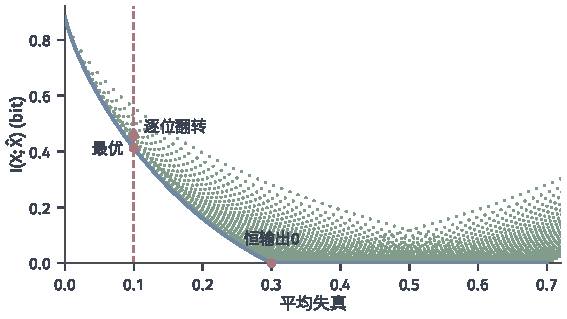
\includegraphics[width=96mm]{figures/07-probability/05-source-coding/matplotlib/rd-test-channel-cloud/figure.pdf}
  \caption{$\operatorname{Bern}(0.3)$信源与Hamming失真下全部二元测试信道的平均失真与互信息。绿点：$q(1\mid0)$与$q(0\mid1)$各取$0,\tfrac1{60},\dots,1$共$61\times61$个组合。蓝线是点云的下边界$R(D)$，其公式在第~\ref{sec:rd-binary}节导出。红点依次是以$0.1$翻转的测试信道、$D=0.1$时的最优测试信道和恒输出$0$；红色虚线是$D=0.1$。}
  \label{fig:rd-test-channel-cloud}
\end{BookInlineFigure}

\subsection{单调性与凸性}
\label{sec:rd-convexity}

点云的下边界看上去单调下降、向下凸。单调性只需比较可行集合。

失真预算放宽时，满足$\mathbb{E}d\leq D$的测试信道都满足$\mathbb{E}d\leq D'$，其中$D<D'$。在更大的集合上取下确界只会更小，所以$R(D')\leq R(D)$，$R$非增。

凸性来自互信息对测试信道的凸性。证明要用一个关于两组非负数的不等式，它把KL散度非负的论证推广到未归一化的数组。

\begin{lemma}[对数和不等式]
\label{lem:rd-log-sum}
设$a_1,\dots,a_k\geq0$，$b_1,\dots,b_k>0$，$a=\sum_ia_i$，$b=\sum_ib_i$。则
\begin{equation}
  \sum_{i=1}^{k}a_i\log_2\frac{a_i}{b_i}\geq a\log_2\frac{a}{b},
  \label{eq:rd-log-sum}
\end{equation}
约定$0\log_20=0$。
\end{lemma}

\begin{proof}
$a=0$时两边都为$0$。设$a>0$，记$\phi(t)=t\log_2t$（$\phi(0)=0$），它在$[0,\infty)$上凸，因为$t>0$时$\phi''(t)=1/(t\ln2)>0$。左端可以写成
\[
  \sum_{i}a_i\log_2\frac{a_i}{b_i}=b\sum_{i}\frac{b_i}{b}\,\phi\Bigl(\frac{a_i}{b_i}\Bigr).
\]
权重$b_i/b$非负且和为$1$，由Jensen不等式，
\[
  \sum_{i}\frac{b_i}{b}\,\phi\Bigl(\frac{a_i}{b_i}\Bigr)\geq\phi\Bigl(\sum_{i}\frac{b_i}{b}\cdot\frac{a_i}{b_i}\Bigr)=\phi\Bigl(\frac{a}{b}\Bigr)=\frac{a}{b}\log_2\frac{a}{b}.
\]
两边乘以$b$即得式~\eqref{eq:rd-log-sum}。
\end{proof}

\begin{lemma}[互信息对测试信道的凸性]
\label{lem:rd-mi-convex}
固定有限字母表上的源分布$P_X$。对测试信道$q_1,q_2$与$\lambda\in[0,1]$，令$q_\lambda=\lambda q_1+(1-\lambda)q_2$，则
\begin{equation}
  I(P_X,q_\lambda)\leq\lambda\,I(P_X,q_1)+(1-\lambda)\,I(P_X,q_2).
  \label{eq:rd-mi-convex}
\end{equation}
\end{lemma}

\begin{proof}
$q_\lambda$的每一行仍是概率分布，所以它是测试信道。固定一对$(x,\hat{x})$，记
\[
  a_j=p(x)\,q_j(\hat{x}\mid x),\qquad b_j=p(x)\,r_{q_j}(\hat{x}),\qquad j=1,2 .
\]
由式~\eqref{eq:rd-output-marginal}，$r_q$对$q$是线性的，所以$q_\lambda$对应的两个量正好是$\lambda a_1+(1-\lambda)a_2$与$\lambda b_1+(1-\lambda)b_2$。

式~\eqref{eq:rd-test-information}在$(x,\hat{x})$处的项是$a\log_2(a/b)$的形式。对两项$\lambda a_1,(1-\lambda)a_2$与$\lambda b_1,(1-\lambda)b_2$用引理~\ref{lem:rd-log-sum}（分母为零的项分子也为零，可以略去），得
\[
  \bigl(\lambda a_1+(1-\lambda)a_2\bigr)\log_2\frac{\lambda a_1+(1-\lambda)a_2}{\lambda b_1+(1-\lambda)b_2}
  \leq\lambda\,a_1\log_2\frac{a_1}{b_1}+(1-\lambda)\,a_2\log_2\frac{a_2}{b_2}.
\]
对所有$(x,\hat{x})$求和，左端是$I(P_X,q_\lambda)$，右端是式~\eqref{eq:rd-mi-convex}的右端。
\end{proof}

\begin{theorem}[$R(D)$的单调性与凸性]
\label{thm:rd-convex}
有限字母表上，$R$在$[0,\infty)$上非增。在$R$取有限值的区间上，对任意$D_1,D_2$与$\lambda\in[0,1]$，
\begin{equation}
  R\bigl(\lambda D_1+(1-\lambda)D_2\bigr)\leq\lambda R(D_1)+(1-\lambda)R(D_2).
  \label{eq:rd-convex}
\end{equation}
\end{theorem}

\begin{proof}
非增性已经说明。取$\varepsilon>0$，按下确界的定义取测试信道$q_1,q_2$，使
\[
  \mathbb{E}_{q_j}d\leq D_j,\qquad I(P_X,q_j)\leq R(D_j)+\varepsilon,\qquad j=1,2 .
\]
式~\eqref{eq:rd-test-distortion}对$q$是线性的，所以$q_\lambda$的平均失真是
\[
  \lambda\,\mathbb{E}_{q_1}d+(1-\lambda)\,\mathbb{E}_{q_2}d\leq\lambda D_1+(1-\lambda)D_2 ,
\]
$q_\lambda$在后者的可行集合中。

由$R$的定义与引理~\ref{lem:rd-mi-convex}，
\[
  R\bigl(\lambda D_1+(1-\lambda)D_2\bigr)\leq I(P_X,q_\lambda)
  \leq\lambda R(D_1)+(1-\lambda)R(D_2)+\varepsilon .
\]
令$\varepsilon\to0$即得式~\eqref{eq:rd-convex}。
\end{proof}

证明中把两个测试信道按比例混合：对每个输入，先以概率$\lambda$决定用$q_1$还是$q_2$，再按选中的那个重构。失真随混合线性变化，互信息却至多线性变化，这就是凸性。

块编码中的分时是同一想法的操作版本。设两列码分别达到$(R_1,D_1)$与$(R_2,D_2)$。块长为$n$时，前$\lfloor\lambda n\rfloor$个符号用第一列中相应块长的码，其余符号用第二列的码，编号合起来发送。码率与失真都按符号比例加权，趋于$\lambda R_1+(1-\lambda)R_2$与$\lambda D_1+(1-\lambda)D_2$，所以可达区域也是凸的。

图~\ref{fig:rd-convexity}比较这两种混合。$q_1$是照传，$q_2$是恒输出$0$，各取一半。混合后的测试信道在$X=0$时输出$0$，在$X=1$时以$\tfrac12$的概率输出$1$，失真为$0.15$。由$r_q(1)=0.15$与$H(\hat{X}\mid X)=0.3\,h_2(\tfrac12)$，它的互信息是
\[
  I=h_2(0.15)-0.3\approx0.6098-0.3=0.3098 .
\]
这低于两端点连线在$D=0.15$处的高度$0.4406$。同样比例的分时只能落在连线上，混合测试信道已经越过了它；而$R(0.15)\approx0.2715$又比混合更低。

\begin{BookInlineFigure}
  \centering
  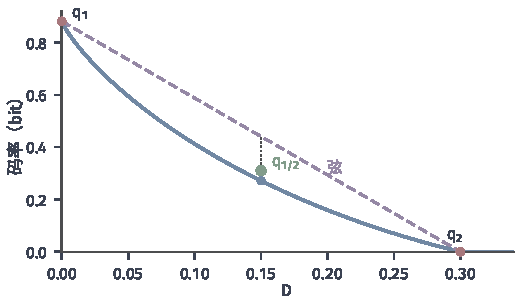
\includegraphics[width=88mm]{figures/07-probability/05-source-coding/matplotlib/rd-convexity/figure.pdf}
  \caption{$\operatorname{Bern}(0.3)$与Hamming失真下$R(D)$的凸性。红点$q_1$是照传（$D=0$，$I=h_2(0.3)$），$q_2$是恒输出$0$（$D=0.3$，$I=0$），紫色虚线是两者之间的弦，也是分时所能达到的点。绿点是两个测试信道各占一半的混合，高$0.3098$，蓝点是同一失真$0.15$下的$R(0.15)\approx0.2715$。}
  \label{fig:rd-convexity}
\end{BookInlineFigure}

\subsection{可行范围与零码率失真}
\label{sec:rd-feasible-range}

$R(D)$在哪些$D$上有限，在哪里降到零？下确界能否取到？这些问题决定了曲线的两个端点，也为编码定理的证明提供需要的连续性。本小节先设$\mathcal{X}$与$\hat{\mathcal{X}}$有限，$d$取非负有限值。

\paragraph{最小可行失真}
任何测试信道的平均失真都不会低于“每个源值都用它最好的重构”时的失真。对每个$x$，$d(x,\cdot)$按$q(\cdot\mid x)$的平均不小于它的最小值，再按$p(x)$平均得到$\mathbb{E}d\geq D_{\min}$，其中
\begin{equation}
  D_{\min}=\sum_{x}p(x)\min_{\hat{x}}d(x,\hat{x}).
  \label{eq:rd-dmin}
\end{equation}
把每个$x$确定地送到一个使$d(x,\cdot)$最小的$\hat{x}$，就达到$D_{\min}$。所以$D<D_{\min}$时可行集合为空，$R(D)=+\infty$；$D\geq D_{\min}$时可行集合非空。

另一端，若$\hat{X}$与$X$独立，平均失真是对重构边缘$r$的加权平均：
\[
  \mathbb{E}d=\sum_{\hat{x}}r(\hat{x})\sum_{x}p(x)d(x,\hat{x})\geq\min_{\hat{x}}\sum_{x}p(x)d(x,\hat{x}).
\]
右端记为
\begin{equation}
  D_{\max}=\min_{\hat{x}\in\hat{\mathcal{X}}}\sum_{x}p(x)\,d(x,\hat{x}),
  \label{eq:rd-dmax}
\end{equation}
它是只输出一个最佳常量时的失真，称为\term{零码率失真}（zero-rate distortion）。只输出一个常量不需要任何描述，所以$D\geq D_{\max}$时$R(D)=0$。

\begin{theorem}[最优测试信道的存在与$R$的连续性]
\label{thm:rd-existence}
设$\mathcal{X},\hat{\mathcal{X}}$有限，$d$非负有限。对每个$D\geq D_{\min}$，式~\eqref{eq:rd-information-rd}中的下确界可以取到，并且$R(D)\leq H(X)$。$R$在$[D_{\min},\infty)$上连续。
\end{theorem}

\begin{proof}
把测试信道看成$\mathbb{R}^{\lvert\mathcal{X}\rvert\times\lvert\hat{\mathcal{X}}\rvert}$中的矩阵。各行非负且和为$1$的矩阵组成有界闭集，式~\eqref{eq:rd-test-distortion}对$q$线性，$\mathbb{E}d\leq D$是一个闭的半空间。两者之交$\mathcal{Q}(D)$是非空紧集。

互信息对$q$连续。把式~\eqref{eq:rd-test-information}中的对数拆开，并按式~\eqref{eq:rd-output-marginal}合并$\hat{x}$相同的项，得
\[
  I(P_X,q)=\sum_{x,\hat{x}}p(x)\,\phi\bigl(q(\hat{x}\mid x)\bigr)-\sum_{\hat{x}}\phi\bigl(r_q(\hat{x})\bigr),
\]
其中$\phi(t)=t\log_2t$在$[0,1]$上连续，$r_q$对$q$线性。连续函数在非空紧集上取到最小值，所以下确界可以取到。又$I(P_X,q)\leq H(X)$对一切$q$成立，因为$I=H(X)-H(X\mid\hat{X})$，故$R(D)\leq H(X)$。

连续性先看内部。$R$在$[D_{\min},\infty)$上取有限值并且是凸函数，开区间上的凸函数连续，所以$R$在$(D_{\min},\infty)$上连续。

在端点$D_{\min}$处，取$D_k\downarrow D_{\min}$与相应的最优测试信道$q_k\in\mathcal{Q}(D_k)$。所有$q_k$落在紧集$\mathcal{Q}(D_1)$中，取收敛子列$q_{k_j}\to q$。由失真的线性与连续性，$q$的平均失真不超过$D_{\min}$，于是
\[
  R(D_{\min})\leq I(P_X,q)=\lim_{j\to\infty}R(D_{k_j}).
\]
另一方面$R$非增，$R(D_{k_j})\leq R(D_{\min})$。两边夹住，$R(D_k)\to R(D_{\min})$。
\end{proof}

\begin{theorem}[零码率失真]
\label{thm:rd-zero-rate}
在定理~\ref{thm:rd-existence}的条件下，$R(D)=0$当且仅当$D\geq D_{\max}$。在$[D_{\min},D_{\max}]$上$R$严格递减。
\end{theorem}

\begin{proof}
$D\geq D_{\max}$时恒输出最佳常量可行，互信息为零。反之设$R(D)=0$，由定理~\ref{thm:rd-existence}，存在可行的$q$使$I(P_X,q)=0$，即$X$与$\hat{X}$独立。由式~\eqref{eq:rd-dmax}前的计算，它的平均失真至少为$D_{\max}$，所以$D\geq D_{\max}$。

严格递减用反证。设$D_{\min}\leq D_1<D_2\leq D_{\max}$且$R(D_1)=R(D_2)$。由刚证明的结论，$D_1<D_{\max}$蕴含$R(D_1)>0$。若$D_2<D_{\max}$，把$D_2$写成$D_1$与$D_{\max}$的凸组合$D_2=\lambda D_1+(1-\lambda)D_{\max}$，$\lambda\in(0,1)$，由式~\eqref{eq:rd-convex}，
\[
  R(D_2)\leq\lambda R(D_1)+(1-\lambda)\cdot0<R(D_1),
\]
其中最后一步用了$R(D_1)>0$，与假设矛盾。若$D_2=D_{\max}$，则$R(D_1)=0$，与$D_1<D_{\max}$矛盾。
\end{proof}

当$\mathcal{X}=\hat{\mathcal{X}}$且$d(x,\hat{x})=0$当且仅当$x=\hat{x}$时，$D_{\min}=0$，而$\mathbb{E}d=0$迫使$\hat{X}=X$，于是$R(0)=I(X;X)=H(X)$。零失真的码率回到第~\ref{chap:lossless-coding}章的熵。雨天记录的例子中$D_{\min}=0$，$R(0)=h_2(0.3)$；零码率失真$D_{\max}=\min\{0.3,0.7\}=0.3$，就是一律猜“不下雨”。

\paragraph{一个$D_{\min}>0$的例子}
设$X$在$\{0,1,2\}$上取值，概率为$(0.3,0.4,0.3)$，而重构只能取$\hat{\mathcal{X}}=\{0,2\}$，失真为平方误差。$x=1$离两个重构值都是$1$，所以由式~\eqref{eq:rd-dmin}，
\[
  D_{\min}=0.4\times1=0.4 .
\]
两个常量重构的平均失真都是$0.4\times1+0.3\times4=1.6$，所以$D_{\max}=1.6$。

$D=D_{\min}$时，$0$必须重构为$0$，$2$必须重构为$2$，否则会多出$4$的失真；只有$x=1$可以自由选择。设它以概率$a$重构为$2$，则$\mathbb{P}(\hat{X}=2)=0.3+0.4a$，$H(\hat{X}\mid X)=0.4\,h_2(a)$，
\[
  I(a)=h_2(0.3+0.4a)-0.4\,h_2(a).
\]

用$h_2'(t)=\log_2\frac{1-t}{t}$求导，
\[
  I'(a)=0.4\log_2\frac{0.7-0.4a}{0.3+0.4a}-0.4\log_2\frac{1-a}{a}.
\]
令其为零，得$a(0.7-0.4a)=(1-a)(0.3+0.4a)$，展开后$0.7a=0.3+0.1a$，即$a=\tfrac12$。$I$是测试信道的凸函数，在这条线段上也凸，所以这是最小点：
\[
  R(D_{\min})=I\Bigl(\frac12\Bigr)=h_2(0.5)-0.4=0.6 .
\]
对照$a=0$时的$h_2(0.3)\approx0.881$与源熵$H(X)\approx1.571$：零失真不可行，在最小失真处也不必把源描述得一清二楚，那个处在中间、怎样重构都一样差的符号正好用来“抛硬币”。

图~\ref{fig:rd-ternary-range}画出这个例子的整条曲线。左侧浅红区域不可行；曲线从$(0.4,0.6)$开始，严格下降，在$D_{\max}=1.6$处降到零，之后保持为零。

\begin{BookInlineFigure}
  \centering
  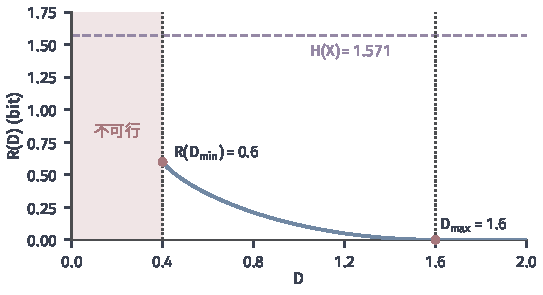
\includegraphics[width=92mm]{figures/07-probability/05-source-coding/matplotlib/rd-ternary-range/figure.pdf}
  \caption{三元信源$p=(0.3,0.4,0.3)$、重构字母表$\{0,2\}$与平方失真的$R(D)$（蓝线），由第~\ref{sec:rd-computation}节的算法逐点计算。浅红区域$D<D_{\min}=0.4$不可行；红点是$(D_{\min},0.6)$与$(D_{\max},0)$；紫色虚线是源熵$H(X)\approx1.571$\,bit。}
  \label{fig:rd-ternary-range}
\end{BookInlineFigure}

\paragraph{一般重构空间}
重构值取实数或其他无限集合时，上面每一步都要重新核对。$d$需要对乘积$\sigma$代数可测，平均失真才有定义；可行的Markov核要组成某种意义下的紧集，互信息要对这种收敛下半连续，下确界才能取到。这些条件并不自动成立。

设$X\sim\operatorname{Bern}(\tfrac12)$，重构只能取开区间$(0,1)$中的值，$d(x,\hat{x})=\lvert x-\hat{x}\rvert$。把式~\eqref{eq:rd-dmin}中的最小值换成下确界，$D_{\min}$仍是$0$，但没有重构值能让失真为零，平均失真为$0$的测试信道不存在，$R(0)=+\infty$。

另一方面，对任意$\varepsilon\in(0,\tfrac12)$，把$0$重构为$\varepsilon$、把$1$重构为$1-\varepsilon$，平均失真为$\varepsilon$，互信息为$1$。所以$R(D)\leq1$对一切$D>0$成立，$R$在$0$处从有限值跳到$+\infty$。这里$\hat{\mathcal{X}}$不紧，下确界“存在”只是一个数，最优重构并未取到，定理~\ref{thm:rd-existence}的结论也随之失效。
